\documentclass[conference]{IEEEtran}


\usepackage[utf8]{inputenc}
\usepackage[x11names]{xcolor}

\usepackage[np]{numprint}

\definecolor{linkcolor}{RGB}{36,113,163}
\definecolor{citecolor}{RGB}{17,122,101}
\definecolor{urlcolor}{RGB}{148,39,38}

\usepackage[
    colorlinks,
    linkcolor=linkcolor,
    citecolor=citecolor,
    urlcolor=urlcolor
]{hyperref}

\usepackage{algorithm}
\usepackage{algpseudocode}

\usepackage{amsmath, amsfonts}

\usepackage{lipsum}

\usepackage{tikz}
\usetikzlibrary{decorations.pathreplacing, patterns}
\usetikzlibrary{calc, backgrounds}

\usepackage{xspace}

\usepackage{listings}
\usepackage{cleveref}

\lstset{
    basicstyle=\ttfamily,
    keywordstyle={[1]\color{Blue4}\bfseries}, % keywords style
    % keywordstyle={[2]\color{Pink4}}, % type style
    % keywordstyle={[3]\color{OrangeRed3}}, % function style
    % literate =
    %     {=>}{{=>}}2
    %     {/=}{{/=}}2,
    commentstyle=\itshape\color{gray}
}

\def\spark#1{\lstinline[language=Ada]{#1}}

\usepackage{todonotes}
%\def\todo#1{\textcolor{red}{[#1]}}

\def\state#1{\textsf{\MakeUppercase{#1}}\xspace}
\def\sclosed{\state{closed}}
\def\ssynsent{\state{syn-sent}}
\def\ssynrcv{\state{syn-rcvd}}
\def\slisten{\state{listen}}
\def\sestab{\state{established}}
\def\sfwone{\state{fin-wait-1}}
\def\sfwtwo{\state{fin-wait-2}}
\def\sclosing{\state{closing}}
\def\sclosew{\state{close-wait}}
\def\slastack{\state{last-ack}}
\def\stimewait{\state{time-wait}}

\def\flag#1{\textsf{#1}\xspace}
\def\syn{\flag{SYN}}
\def\ack{\flag{ACK}}
\def\rst{\flag{RST}}
\def\fin{\flag{FIN}}

\let\code\texttt

\begin{document}

\title{Layered Formal Verification of an Industrial TCP/IP Stack}

\author{%
\IEEEauthorblockN{Guillaume Cluzel}
\IEEEauthorblockA{\textit{AdaCore \& ENS de Lyon}}
\and
\IEEEauthorblockN{Kyriakos Georgious}
\IEEEauthorblockA{\textit{AdaCore \& University of Bristol}}
\and
\IEEEauthorblockN{Yannick Moy}
\IEEEauthorblockA{\textit{AdaCore}}
\and
\IEEEauthorblockN{Clément Zeller}
\IEEEauthorblockA{\textit{Oryx Embedded}}
}

\maketitle

\begin{abstract}
\todo{Write the abstract.}
\end{abstract}

\begin{IEEEkeywords}
Network protocols,
deductive verification.
\end{IEEEkeywords}

\section{Introduction}

By 2030 it is estimated that one trillion Internet of Things (IoT) devices will be deployed and be part of every aspect of our daily life~\cite{IoT_route:ARM_white_paper}. At the same time, it is made evident that security for such systems is a major challenge~\cite{Sec_IoT_Challenges:paper,Cyber_Systems_security:paper}. Any vulnerability in software libraries that are widely used by embedded systems can potentially open the door for compromising the security of billions of deployed IoT devices. Researchers have shown that such vulnerabilities exist: in 2019, critical security vulnerabilities were discovered in a TCP implementation that has been used by billions of IoT devices for more than 13 years~\cite{zero_days_vuln:ARMIS_white_paper}, some of them allowing remote code execution.

Networking communication models define the processes of transferring information from one network component to another. Currently, the two most popular networking communication models are the TCP/IP (Transmission Control Protocol/Internet Protocol) \cite{TCP_IP:ietf_tutorial} and the OSI (Open System Interconnection) \cite{ISO:35.100} models. Layering is an essential design requirement for both models to achieve modularity, flexibility, and abstraction. Applications that only need to use the lower levels' functionality can drop all the unnecessary upper levels. \Cref{Fig:TcpStack} shows the various layers of the OSI model. Each layer supports a wide range of protocols that are compatible with the layer's specifications. The lowest layers, bottom layers in \Cref{Fig:TcpStack}, are more hardware-oriented, while the top layers are more software-specific. While the \emph{application} level has a wide range of protocols that can be used depending on the application specification, the \emph{transport} layer is heavily dependent on the two dominant protocols: Transmission Control Protocol (TCP) and User Datagram Protocol (UDP). Today, almost every networking application, including IoT devices, is using either the TCP or the UDP protocols to traffic data between the Network and the Application layers. %Thus, the reliability, assurance, and security of these protocols are of paramount importance for critical applications.

\newlength\hatchdistance
\hatchdistance=10pt
\pgfdeclarepatternformonly[\hatchdistance,2pt]{north east hatch}% name
    {\pgfqpoint{-1pt}{-1pt}}% below left
    {\pgfqpoint{\hatchdistance}{\hatchdistance}}% above right
    {\pgfpoint{\hatchdistance-1pt}{\hatchdistance-1pt}}%
    {
        \pgfsetcolor{orange!40}
        \pgfsetlinewidth{2pt}
        \pgfpathmoveto{\pgfqpoint{0pt}{0pt}}
        \pgfpathlineto{\pgfqpoint{\hatchdistance}{\hatchdistance}}
        \pgfusepath{stroke}
    }
\begin{figure}[t]
    \centering\begin{tikzpicture}[x=.12\linewidth,y=.45cm,
        application/.style={font=\sffamily\tiny,
                            draw,
                            minimum width=.115\linewidth,
                            minimum height=.4cm},
        session/.style={font=\sffamily\tiny,
                        draw,
                        minimum width=.715\linewidth,
                        minimum height=.4cm},
        transport/.style={font=\sffamily\tiny,
                          draw,
                          minimum width=.295\linewidth,
                          minimum height=.4cm},
        network/.style={font=\sffamily\tiny,
                        draw,
                        minimum width=.355\linewidth,
                        minimum height=.4cm},
        datalink/.style={font=\sffamily\tiny,
                         draw,
                         minimum width=.139\linewidth,
                         minimum height=.4cm}
    ]
        \node[application] at (0,10) {HTTP};
        \node[application] at (1,10) {HTTP/2};
        \node[application] at (2,10) {MQTT};
        \node[application] at (3,10) {MQTT-SN};
        \node[application] at (4,10) {CoAP};
        \node[application] (CoinA) at (5,10) {FTP};
        \node[application] at (0,9)  {SMTP};
        \node[application] at (1,9)  {SNTP};
        \node[application] at (2,9)  {DNS};
        \node[application] at (3,9)  {NetBIOS};
        \node[application] at (4,9)  {SNMPv3};
        \node[application] at (5,9)  {TFTP};
        \node[application, minimum width=.235\linewidth] at (.5,8) {WebSocket};
        \node[application] at (2,8)  {mDNS};
        \node[application] at (3,8)  {DNS-SD};
        \node[application] at (4,8)  {DHCP};
        \node[application] (CoinB) at (5,8)  {DHCPv6};
        \node[session, fill=green!70!yellow!20] (Socket) at (2.5, 7) {Socket};
        \node[transport, preaction={fill, green!70!yellow!20}, pattern=north east hatch, pattern color=orange!40] at (.75,6) {TCP};
        \node[transport, fill=orange!40] at (3.25,6) {UDP};
        \node[application, fill=orange!40] (RAW) at (5,6) {RAW};
        \node[network, fill=orange!40] at (1, 5) {IPv4};
        \node[network, fill=orange!40] (IPv6) at (4, 5) {IPv6};
        \node[application, fill=orange!40] at (0,4) {ARP};
        \node[application, fill=orange!40] at (1,4) {Auto-IP};
        \node[application, fill=orange!40] at (2,4) {NDP};
        \node[application, fill=orange!40] at (3,4) {SLAAC};
        \node[application, fill=orange!40] (ICMP) at (4,4) {ICMP};
        \node[application, fill=orange!40] (MLDv1) at (5,4) {MLDv1};
        \node[datalink, fill=orange!40] at (0.10, 3) {Ethernet};
        \node[datalink, fill=orange!40] at (1.3, 3) {Wi-Fi};
        \node[datalink, fill=orange!40] at (2.5, 3) {PPP};
        \node[datalink, fill=orange!40] at (3.7, 3) {USB/RNDIS};
        \node[datalink, fill=orange!40] (G3) at (4.9, 3) {G3-PLC};


        \draw[decorate, decoration={brace}, line width=.5pt]
            ([xshift=2pt]CoinA.north east) -- ([xshift=2pt]CoinB.south east)
            node [midway, anchor=west, font=\sffamily\tiny] {Application layer};
        \draw[decorate, decoration={brace}, line width=.5pt]
            ([xshift=2pt]Socket.north east) -- ([xshift=2pt]Socket.south east)
            node [midway, anchor=west, font=\sffamily\tiny] {Session layer};
        \draw[decorate, decoration={brace}, line width=.5pt]
            ([xshift=2pt]RAW.north east) -- ([xshift=2pt]RAW.south east)
            node [midway, anchor=west, font=\sffamily\tiny] {Transport layer};
        \draw[decorate, decoration={brace}, line width=.5pt]
            ([xshift=2pt]IPv6.north east) -- ([xshift=2pt]MLDv1.south east)
            node [midway, anchor=west, font=\sffamily\tiny] {Network layer};
        \draw[decorate, decoration={brace}, line width=.5pt]
            ([xshift=2pt]G3.north east) -- ([xshift=2pt]G3.south east)
            node [midway, anchor=west, font=\sffamily\tiny] {Data Link layer};
    \end{tikzpicture}

    \caption{Overview of the TCP/IP CycloneTCP stack in the OSI model. Green parts represent
             what have been translated in SPARK and in orange the underlying untrusted part written in C.}
    \label{Fig:TcpStack}
\end{figure}

Existing research has dealt with formally verifying several protocols of TCP/IP stack levels. Early work formalized the TCP protocol to prove some key properties of the protocol itself~\cite{smith1996formal}. More recently, researchers have formally specified TCP, UDP and the Sockets API in HOL~\cite{tcp2005sigcomm,ridge2008rigorous} and used the resulting specification for testing existing libraries. Others have formally specified and implemented the SSL/TLS protocol in F*\cite{bhargavan2013implementing}, and integrated the resulting implementation in existing libraries. To the best of our knowledge, no prior work attempted to formally verify an implementation of TCP, although the authors of~\cite{ridge2008rigorous} suggest that it would possible to extract an actual implementation in Haskell from their specification.

In this paper, we take a practical approach, where the security of an existing TCP/IP stack implementation written in ANSI C programming language is incrementally enhanced by replacing parts of its code with formally verified code in SPARK~\cite{mccormick_chapin_2015}, a subset of the Ada programming language supported by formal verification tools. We chose CycloneTCP, a professional-grade open source embedded TCP/IP library developed by the Oryx Embedded company~\cite{CycloneTCP}. \Cref{Fig:TcpStack} shows the protocols supported by the library. This work focuses on the TCP and Socket components of the stack. The library's TCP implementation is meant to conform with the RFC 793 protocol specifications~\cite{rfc793}. The quality of the CycloneTCP is acknowledged by the AMNESIA:33 report~\cite{AMNESIA33}, which classifies it as one of the most resilient TCP/IP stack.

In total, for this work, 50 subprograms have been translated from C to SPARK. This accounts for 2266 lines of code, of which 1165 are SPARK logic code (e.g\.~ contracts) used to represent and prove the protocol's specification. The overall proving time with GNATprove is 9m and 54s on a 12-processor Intel(R) Core(TM) i7-9750H CPU with 2.60GHz speed and 16GB of RAM.

\todo[inline]{KG:pending contributions list and fixing the next paragraph. Will be fixed when the rest of the paper is finalized.}

We present the TCP protocol in section~\ref{sec:TCP} and then briefly the
chosen stack, the Oryx Embedded one, in section~\ref{sec:stack}
before presenting the specification techniques used in section~\ref{sec:spec}
and then in sections~\ref{sec:verif} and~\ref{sec:API} we explain how we
formally implemented in SPARK the TCP user functions and how we hardened the
user's API. Finally we end in section~\ref{sec:results} by showing the results
of our work.

\section{Overview of the TCP protocol specification}
\label{sec:TCP}


\begin{figure}[t]
    {\centering\scalebox{.55}{
    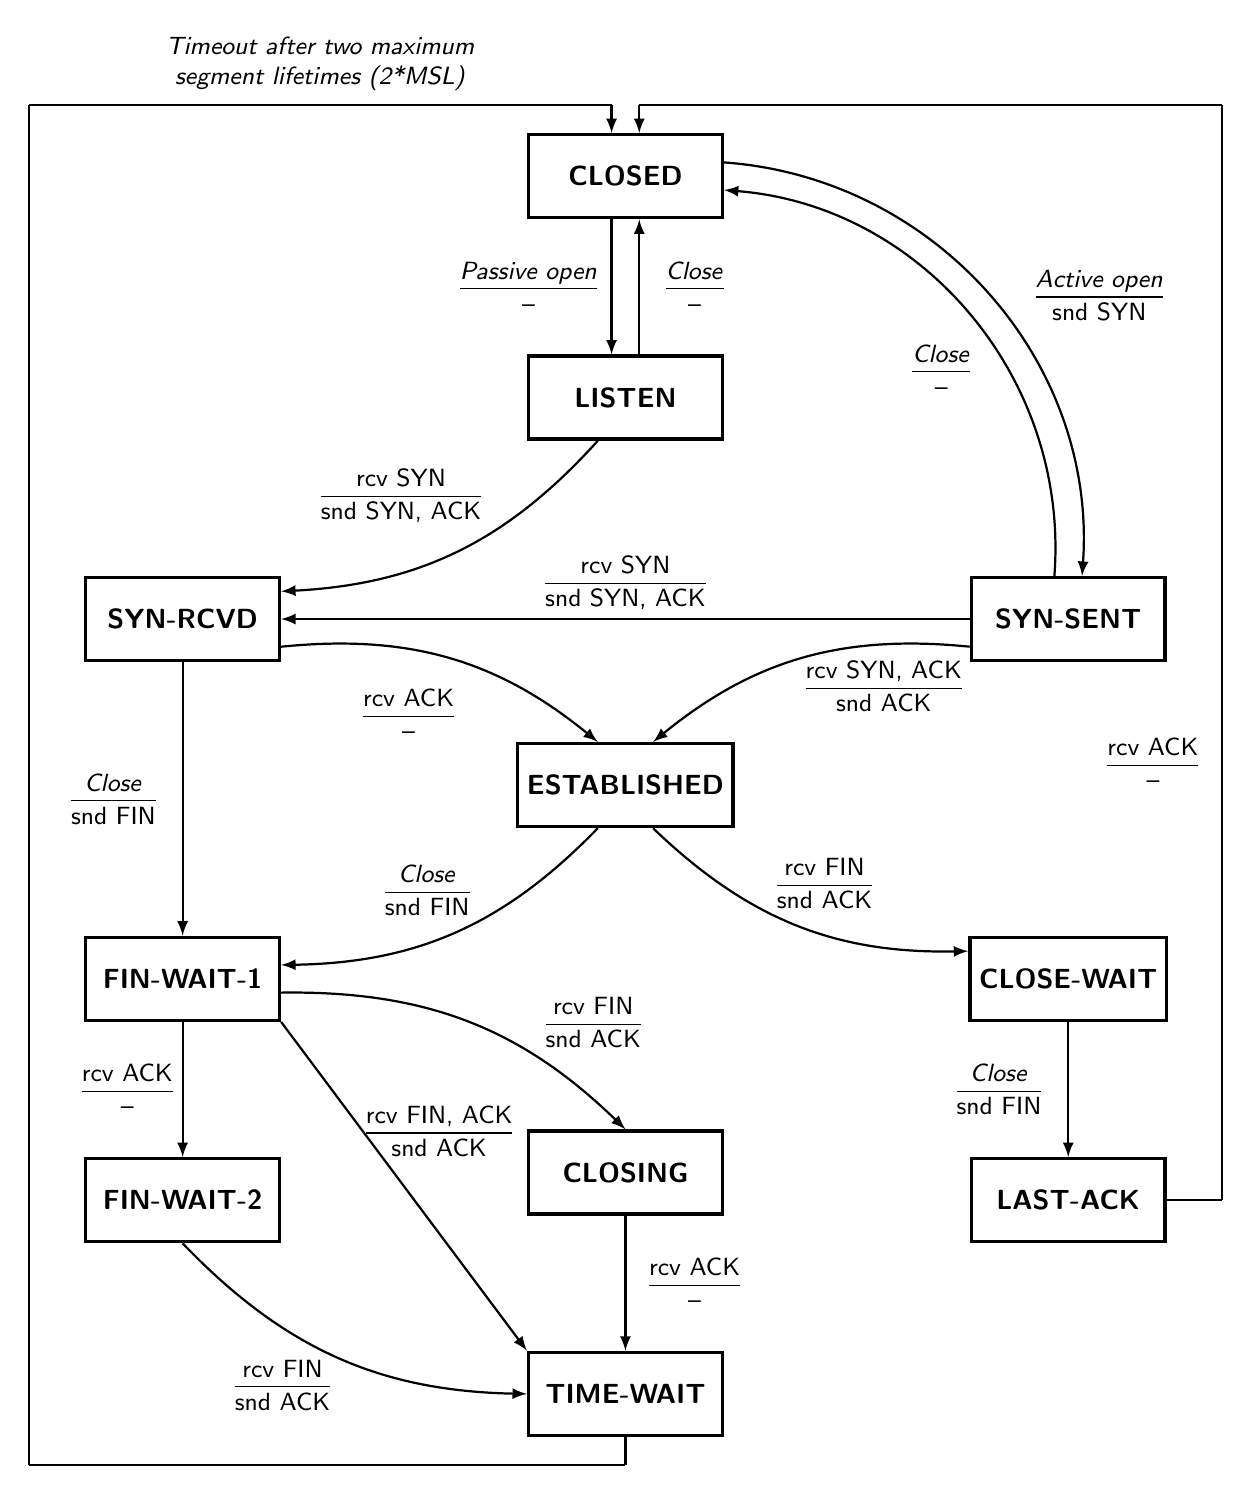
\begin{tikzpicture}[>=latex]
        \def\tfrac#1#2{\ensuremath{\displaystyle\frac{\text{\small#1}}{\text{\small#2}}}}
        %
        % Styles for states, and state edges
        %
        \tikzstyle{state} = [draw, very thick, fill=white, rectangle, minimum height=3em, minimum width=7em, node distance=8em, font={\sffamily\bfseries}]
        \tikzstyle{stateEdgePortion} = [black,thick];
        \tikzstyle{stateEdge} = [stateEdgePortion,->];
        \tikzstyle{edgeLabel} = [pos=0.5, text centered, font={\sffamily\small}];

        %
        % Position States
        %
        \node[state, name=closedStart] {CLOSED};
        \node[state, name=listen, below of=closedStart] {LISTEN};
        \node[state, name=synSent, below of=listen, right of=listen, xshift=8em] {SYN-SENT};
        \node[state, name=synRcvd, below of=listen, left of=listen, xshift=-8em] {SYN-RCVD};
        \node[state, name=established, below of=listen, node distance=14em] {ESTABLISHED};
        \node[state, name=finWait1, below of=established, left of=established, node distance=7em, xshift=-9em] {FIN-WAIT-1};
        \node[state, name=finWait2, below of=finWait1] {FIN-WAIT-2};
        \node[state, name=closeWait, below of=established, right of=established, node distance=7em, xshift=9em] {CLOSE-WAIT};
        \node[state, name=closing, below of=established, node distance=14em] {CLOSING};
        \node[state, name=lastAck, below of=closeWait] {LAST-ACK};
        \node[state, name=timeWait, below of=closing] {TIME-WAIT};

        %
        % Connect States via edges
        %
        \draw ($(closedStart.south) + (-.5em,0)$)
        edge[stateEdge] node[edgeLabel, xshift=-3em]{\tfrac{\emph{Passive open}}{--}}
        ($(listen.north) + (-.5em,0)$);
        \draw ($(listen.north) + (.5em,0)$)
        edge[stateEdge] node[edgeLabel, xshift=2em]{\tfrac{\emph{Close}}{--}}
        ($(closedStart.south) + (.5em,0)$);

        \draw ($(listen.south) + (-1em,0)$)
        edge[stateEdge, bend left=22.5] node[edgeLabel, xshift=-2em, yshift=2em]{\tfrac{rcv SYN}{snd SYN, ACK}}
        ($(synRcvd.east) + (0,1em)$);

        % \draw ($(synRcvd.north) + (.5em,0)$)
        % edge[stateEdge, bend left=45] node[edgeLabel,xshift=-4em]{\emph{Timeout}/RST}
        % ($(closedStart.west) + (0,-.5em)$);

        \draw ($(synSent.north) + (-.5em,0)$)
        edge[stateEdge, bend right=45] node[edgeLabel,xshift=-1em, yshift=-2em]{\tfrac{\emph{Close}}{--}}
        ($(closedStart.east) + (0,-.5em)$);
        \draw ($(closedStart.east) + (0,.5em)$)
        edge[stateEdge, bend left=45] node[edgeLabel,xshift=4em]{\tfrac{\emph{Active open}}{snd SYN}}
        ($(synSent.north) + (.5em,0)$);

        \draw (synSent.west)
        edge[stateEdge] node[edgeLabel, yshift=1.3em]{\tfrac{rcv SYN}{snd SYN, ACK}}
        (synRcvd.east);
        \draw (synRcvd)
        edge[stateEdge] node[edgeLabel, xshift=-2.5em]{\tfrac{\emph{Close}}{snd FIN}}
        (finWait1);

        \draw ($(synRcvd.east) + (0,-1em)$)
        edge[stateEdge, bend left=22.5] node[edgeLabel, xshift=-1.5em, yshift=-2em]{\tfrac{rcv ACK}{--}}
        ($(established.north) + (-1em,0)$);
        \draw ($(synSent.west) + (0,-1em)$)
        edge[stateEdge, bend right=22.5] node[edgeLabel, xshift=3em, yshift=-1em]{\tfrac{rcv SYN, ACK}{snd ACK}}
        ($(established.north) + (1em,0)$);

        \draw ($(established.south) + (-1em,0)$)
        edge[stateEdge, bend left=22.5] node[edgeLabel, xshift=-1em, yshift=1.5em]{\tfrac{\emph{Close}}{snd FIN}}
        ($(finWait1.east) + (0,.5em)$);
        \draw ($(established.south) + (1em,0)$)
        edge[stateEdge, bend right=22.5] node[edgeLabel, xshift=1em, yshift=1.5em]{\tfrac{rcv FIN}{snd ACK}}
        ($(closeWait.west) + (0,1em)$);

        \draw (finWait1.south)
        edge[stateEdge] node[edgeLabel, xshift=-2em]{\tfrac{rcv ACK}{--}}
        (finWait2.north);
        \draw ($(finWait1.east) + (0,-.5em)$)
        edge[stateEdge, bend left=22.5] node[edgeLabel, yshift=0em, xshift=4.5em]{\tfrac{rcv FIN}{snd ACK}}
        (closing.north);
        \draw (finWait1.south east)
        edge[stateEdge] node[edgeLabel, xshift=0em, yshift=2em, text width=3em]{\tfrac{rcv FIN, ACK}{snd ACK}}
        (timeWait.north west);

        \draw (finWait2.south)
        edge[stateEdge, bend right=22.5] node[edgeLabel, xshift=-2em, yshift=-1em]{\tfrac{rcv FIN}{snd ACK}}
        (timeWait.west);

        \draw (closing)
        edge[stateEdge] node[edgeLabel, xshift=2.5em]{\tfrac{rcv ACK}{--}}
        (timeWait);

        \draw (closeWait)
        edge[stateEdge] node[edgeLabel,xshift=-2.5em]{\tfrac{\emph{Close}}{snd FIN}}
        (lastAck);

        %
        % Connect lastAck to closed is slightly more complicated
        % no direct line-of-sight, so we need to take the scenic route
        %
        \coordinate (lastAck2ClosedA) at ($(lastAck.east) + (2em,0)$);
        \coordinate (lastAck2ClosedB) at ($(closedStart.north -| lastAck.east) + (2em,1em)$);
        \coordinate (lastAck2ClosedC) at ($(closedStart.north) + (0.5em,1em)$);
        \draw (lastAck.east) edge[stateEdgePortion] (lastAck2ClosedA);
        \draw (lastAck2ClosedA) edge[stateEdgePortion] node[edgeLabel,xshift=-2.5em, yshift=-4em]{\tfrac{rcv ACK}{--}} (lastAck2ClosedB);
        \draw (lastAck2ClosedB) edge[stateEdgePortion] (lastAck2ClosedC);
        \draw (lastAck2ClosedC) edge[stateEdge] ($(closedStart.north) + (0.5em,0)$);

        %
        % likewise for timeWait to closed
        %
        \coordinate (timeWait2ClosedA) at ($(timeWait.south) + (0,-1em)$);
        \coordinate (timeWait2ClosedB) at ($(timeWait.south -| finWait2.west) + (-2em,-1em)$);
        \coordinate (timeWait2ClosedC) at ($(closedStart.north -| finWait2.west) + (-2em,1em)$);
        \coordinate (timeWait2ClosedD) at ($(closedStart.north) + (-0.5em,1em)$);
        \draw (timeWait.south) edge[stateEdgePortion] (timeWait2ClosedA);
        \draw (timeWait2ClosedA) edge[stateEdgePortion] (timeWait2ClosedB);
        \draw (timeWait2ClosedB) edge[stateEdgePortion] (timeWait2ClosedC);
        \draw (timeWait2ClosedC) edge[stateEdgePortion]
        node[edgeLabel, text width=12.25em, yshift=1.5em]{\emph{Timeout after two maximum segment lifetimes (2*MSL)}}
        (timeWait2ClosedD);
        \draw (timeWait2ClosedD) edge[stateEdge] ($(closedStart.north) + (-0.5em,0)$);

        % draw dotted lines around passive and active closes
        % \begin{pgfonlayer}{background}
        %     \draw [join=round,black,dotted] ($(closeWait.north west) + (-1em, -1em)$) rectangle ($(lastAck.south east) + (1em, 1em)$);
        %     \draw [join=round,black,dotted] ($(finWait1.north west) + (-1em, -1em)$) rectangle ($(timeWait.south east) + (1em, 1em)$);
        % \end{pgfonlayer}

    \end{tikzpicture}}\par}
    \caption{TCP state machine.}
    \label{Fig:statemachine}
\end{figure}


TCP is a connection-oriented protocol; a connection between the sender and the receiver must be established before transmitting any data. Furthermore, TCP is a reliable protocol since it guarantees the delivery of all the messages and that they are delivered in the order they were sent. It also provides error-checking mechanisms to discard and recover from corrupted data.

%\subsection{TCP state machine}

Generally, every TCP communication session will go through the following three phases (if no error occurs): 1)~opening the connection, 2)~sending and receiving the data, and 3)~closing the connection. The behavior of the three-phase communication can be described by the state machine given in \Cref{Fig:statemachine}. An edge represents a state transition.
An edge-label in the format of $\frac{\ \ x \ \ }{\ \ y \ \ }$ represents the actions associated to the state transition, where $x$ is triggering the transition, and $y$ is produced by the transition.
The trigger $x$ is either an explicit action like \textit{Close}, or the arrival of specific flags, while $y$ always represents the flags transmitted in response to the action that caused the state transition, when present.
An explicit action is either a user-triggered action (through the user's API) or an action automatically triggered by a timeout event. The flags are embedded in the header section of a transmitted segment and can be one of the following:
\begin{itemize}
\item \ack: the last message received by the sender is acknowledged.
\item \syn: this flag is sent to establish a connection.
\item \fin: this flag is sent to close the connection.
\item \rst: this flag is sent to reset the connection, often when an error
occurred on one or the other side.
\end{itemize}

The state machine in \Cref{Fig:statemachine} does not represent the complete protocol specification; for example, it does not reflect error conditions or any actions which are not connected with the state changes. Instead, it gives an overview of all the possible states a TCP connection could reach over its lifetime. Each state has a meaning. \slisten represents waiting for a connection request from any remote TCP and port. \ssynsent and \ssynrcv represent the initialization of the connection that ends when \sestab is reached. \sfwone, \sfwtwo, \sclosing, and \stimewait are a group of states that represent waiting for a connection termination request from the remote TCP. \sclosew and \slastack represent waiting for a connection termination request from the local user. Finally, \sclosed represents no connection state at all.

%\subsection{TCP Multitasking model}

TCP is based on a multitasking model. Different tasks can interact and update the socket data structure, used to retain the status of a TCP connection, to handle the various events that can occur within a TCP session. RFC 793, under Section ``3.9. Event Processing'' page 52, describes a possible implementation of how to handle these events based on three tasks: one for the \emph{user calls}, one for the \emph{arriving segments} and one for the \emph{timers}. The role of each of the three tasks can be summarized as follows. User calls refer to functions, namely \texttt{open}, \texttt{close}, \texttt{abort}, \texttt{send} and \texttt{receive}, that can be called by the user to control the connection, send, or receive data. These functions can trigger transitions between the connection's states since they are intended to control the connection. In the arriving segments task, the received segments are being processed,
and the corresponding messages are sent back. Transitions between states can be triggered on the reception of a segment. Finally, timers control the timeouts, for example, the retransmission timeout to retransmit a message or the time-wait timeout to close the connection after a specified amount of time elapsed. Thus, corresponding transitions to the timeout events can also be triggered by this task. A complete description of the protocol's specification can be found in the RFC 793 document~\cite{rfc793}.

The CycloneTCP implementation adopts the three-task-based model and the socket data structure defined by the RFC 793. Thus, it has tasks dedicated to the user's code, to the timers, and to the processing of incoming segments. Moreover, the user can manipulate a socket through the TCP's library Application Programming Interface (API) to perform various TCP operations, such as data transmission.

\section{Specification techniques used}
\label{sec:spec}

\subsection{The SPARK programming language}

Ada is a general-purpose, procedural programming language that puts great emphasis on the safety and correctness of the program. Some of the safety characteristics of the language are its strong typing system and its extensive compile-time and runtime checks. Common C programming vulnerabilities like using unsafe pointers or improper null termination of strings cannot exist in an Ada program, while issues like buffer overflow or integer overflow can be dynamically captured by Ada’s runtime checks and dealt with via exception handlers. Furthermore, Ada introduced contracts, such as preconditions and postconditions, as part of the language’s standard syntax. Such contracts are vital for explicitly expressing software and verification requirements in the source code to allow for static analyzers or runtime checks to verify that the stated requirements are met.

By subsetting Ada, the SPARK programming language \cite{mccormick_chapin_2015} emerged to provide the largest possible subset of Ada, which is suitable for functional specification and static verification. For instance, in SPARK, expressions should be free from side effects, and aliasing is forbidden (no two variables should share the exact memory location or overlap in memory), including when using pointers thanks to the use of an ownership policy~\cite{dross2020recursive}.

\emph{GNATprove} \cite{GNATProve:users_manual} is the tool that provides formal verification for SPARK through two kinds of analyses. The first enables flow analysis to check the initialization of variables, look at data dependencies between inputs and outputs of subprograms, and detects unused assignments and unmodified variables. The second uses deductive verification to generate verification conditions for SMT solvers via a weakest-precondition calculus to detect possible runtime errors and violations of functional contracts.



\subsection{Interfacing SPARK and C code}

The verification of the entire functional specification of the \emph{CycloneTCP} library is beyond the scope of this work. Instead, the aim is to provide significant security hardening to mostly-C libraries by selective use of SPARK. Thus, this work focuses on the hardening of the TCP library areas that its original authors designated as the most vulnerable or crucial to conform to their functional specifications, namely, the Application Programming Interface (API). This mainly falls under two categories: a) proving the conformance to the protocol's functional specification for the translated code, discussed in \Cref{sec:verif}, and b) hardening the user's API to enforce its correct usage by users, discussed in \Cref{sec:API}.

Ada and SPARK offer an easy-to-use mechanism for interfacing with C code \cite{}. The mechanism allows C-written function to be called by Ada/SPARK code and vice versa and for representing shared data objects. The memory representations of a shared data object must be the same in both the C and the SPARK code. For instance, if a C function is called with a 32-bits integer argument, the SPARK interface of this function should also be called with a 32-bits integer argument. It is the responsibility of the user to ensure this.

Although formal verification can only be applied to the SPARK translated code,  preconditions and postconditions can be attached to C functions interfaced in SPARK to allow reasoning about the side effects of calling these functions by the SPARK code. Since the functional specification of these contracts cannot be proved, it is the programmer's role to ensure their correctness. Interfacing C and SPARK code can be error-prone if it is not done carefully. \Cref{sec:verif} discusses how to mitigate this issue effectively.


\subsection{Dealing with pointers}
\label{sec:pointers}

In the CycloneTCP library, pointers are used both as the type of variables to pass objects when calling other functions and as the type of structure fields; for instance, in the socket structure to store other complex data structures and recursive pointer-based data structures. SPARK uses a pointer ownership model to prevent bugs involving pointers such as memory leak or double free, which imposes some restrictions on how pointers are being manipulated. When a memory area is allocated, a pointer points to this memory area, and thus, it is considered "owned.'' The ownership of the memory can be moved, but the memory must be deallocated before the end of the execution of the program.

\subsection{Specifying the frame condition}

The socket structure is shared between different functions and contains a large number of fields. Most of the fields are used in library parts that are not considered by this work, and thus, are not relevant for our verification. Thus we use \emph{ghost code} in SPARK to focus the verification effort on the relevant subset of the fields, which also makes the specifications easier to write and understand. This is a solution to the classical problem of specifying the \emph{frame condition} for a function, that is, the set of possibly modified objects. \emph{Ghost code} is used by GNATprove for analysis but is not being compiled in the final executable. More specifically, we define a \emph{model} of the actual socket as a ghost function that can be used in contracts: \spark{Model(Sock)} extracts the fields of interest from socket \spark{Sock}. A common usage is within a function postcondition: 

\begin{lstlisting}[language=Ada, basicstyle=\small\ttfamily]
Model(Sock) = (Model(Sock)'Old with delta
                    State => TCP_STATE_CLOSED)
\end{lstlisting}

This states that the fields of \spark{Sock} used by \spark{Model} are not changed when calling the function, except for the field \spark{State} that is equal to \spark{TCP_STATE_CLOSED} after the call.

\section{Conformance to the TCP protocol}
\label{sec:verif}

% The reader can refer to the code at \url{https://github.com/AdaCore/Http_Cyclone}.


\subsection{Extracting a specification from RFC 793}

Extracting a specification is mandatory for providing functional contracts to the user's functions. This can be achieved by interpreting the text of RFC 793. However, the text is underspecified, and thus, only one of the possible implementations is used by this work. The following choices were made in our formalization of the TCP specification:

\begin{itemize}
\item The transitions between states must respect the order given by the
state machine described in figure~\ref{Fig:statemachine}. In particular, a transition from a state to another is valid only if the state machine allows for a transition between these two states.
\item RFC 793 describes the conditions for the state of the socket which need to hold when a user's function is called~\cite[p. 52]{rfc793}. In particular, these conditions specify in what state the function can be called without returning an error. These conditions were turned into preconditions in our formalization.
\end{itemize}

\subsection{Rewriting the TCP user functions}

The original \emph{CycloneTCP} library provides no guarantees that the implementation respects the TCP functional specification. Thus, there is no assurance that the implementation will only allow valid transitions between the different states that a TCP session can exhibit. We aim to use the SPARK technology to verify that the implementation respects the TCP automaton, given in \Cref{Fig:statemachine}. The work is focused on hardening the API of the user task, mainly the high-level user functions, to verify the state transitions. To achieve this, the rest of the TCP protocol, not related to the user task, has to be taken into account. The reason for this is two-fold. First, although user-functions can trigger state transitions, the actual transitions are done by library functions that do not belong to the user-task set of functions. Second, other parts of the library can trigger state transitions during and between the user-task function calls, which can affect the intermediate and final states that a user-related function can exhibit. The TCP user API-related functions were fully translated to SPARK. SPARK bindings were also provided to most of the rest of the library's C functions to allow their invocation from the SPARK code.

RFC 793 document provides all the information needed for the allowed transitions between the different TCP possible states. For any transitions directly triggered by the call of the user-task functions, SPARK contracts, representing transitions allowed by the functional specification, are embedded within the SPARK translated code. The \texttt{TCP\_Change\_State} is a helper function that is called every time a state transition needs to be made to update the socket's state. An incorrect transition allowed by the code will be detected by the prover.

% dire que les fonctions appelées dans le code on était modélisées pour prendre
% en compte les changements d'état TCP qu'elles occasionnent.

% Problème, certains changement d'état se font entre l'appel de deux fonctions,
% ça doit donc être pris en compte. Et certains état se font directement lors de
% l'appel d'une fonction particulière et ça doit aussi être pris en compte.

% Yannick: I don't understand the following, needs to be rephrased if we want to keep it
%
% particular when a new segment is received, it is quite easy to know the
% possible set of state that can have the socket during the all execution of the
% functions.


The concurrent implementation of the TCP protocol allows for multiple interactions between the tasks, synchronous (with a call to \spark{TCP_Wait_For_Events}) or asynchronous (between two user function calls), and thus, numerous possible state changes at any given moment. This makes the functional specification verification significantly challenging, as SPARK does not have a native mode to deal precisely with interactions related to concurrency. To address this, we introduced SPARK functions with contracts that model how the different possible interactions can modify the state of a socket. Finding a correct and precise contract for \spark{TCP_Wait_For_Events} is challenging but needed for the verification of the TCP user functions. The solution is elaborated in the following section.


\subsection{Dealing with synchronous exchanges}

% Yannick: below "a new segement...if it contains a new segment" is not phrased correctly

In the synchronous scenario of interaction between the TCP tasks, the resulting state of a user function can be affected by the rest of the TCP tasks when the user's functions release the mutex to allow for other events to occur. In this case, the function \spark{TCP_Wait_For_Events} (located in the file \texttt{tcp\_misc\_binding.ads}) is called from the user function to check if the event requested is completed. For example, the \spark{TCP_Connect} user function calls \spark{TCP_Wait_For_Events} to wait for the completion of the socket connection event, namely the \spark{SOCKET\_EVENT\_CONNECTED}. The call to the \spark{TCP_Wait_For_Events} releases the mutex, and when the \emph{arriving} task receives the appropriate segments, in this case, a segment with the \syn flag, the connection will be established. This will move the socket to the \sestab state. In the meantime, the \spark{TCP\_Update\_Events} function is monitoring for any state changes, and when it notices that the connection is established, it will trigger the \spark{SOCKET\_EVENT\_CONNECTED} event, using the OS event mechanism. This will allow the \spark{TCP\_Connect} user function to resume execution.


% Yannick: the above final sentence is unclear: what is triggered?

% Yannick: the caption below used the term "user-task related function" which is used nowhere else

\begin{algorithm}[t]
    \caption{Function to compute the possible state after the completion of a
particular event that is requested by a user function.}
\label{algo:waitForEvents}
\begin{algorithmic}[1]
\footnotesize
\Function{TCP\_Wait\_For\_Events\_Proof}{Socket, Event\_Mask}
    \State $S_{last} := \text{Socket}$
    \State $E :=$ \spark{TCP_Update_Events}($S_{last}$)
    \If{$(E\ \&\ \text{Event\_Mask}) \neq 0$}
        \State \textbf{return}  $S_{last}$
    \EndIf
    \For{$i=1$ \textbf{to} $3$}
        \State $S_{last} :=$ \spark{TCP_Process_One_Segment}($S_{last}$)
        \State $E :=$ \spark{TCP_Update_Events}($S_{last}$)
        \If{$(E\ \&\ \text{Event\_Mask}) \neq 0$}
            \State \textbf{return} $S_{last}$
        \EndIf
    \EndFor
    \State \textbf{return} $\emptyset$
\EndFunction
\end{algorithmic}
\end{algorithm}

% Yannick: the whole explanation is unclear. We should rephrase to explain that:
% - a suitable contract is added to function \spark{TCP_Wait_For_Events}
% - to make sure this contract is correct, we implement a ghost procedure
%   \spark{TCP_Wait_For_Events_Proof} as shown in Algorithm 1, that models
%   the possible chain of events that occur while waiting, with the same contract
%   as \spark{TCP_Wait_For_Events}. This procedure is proved automatically
%   without even a loop invariant thanks to loop unrolling in GNATprove.

% \todo[inline]{KG to GC : when you are talking about functions you should say where they are located. There will be readers that will want to see the corresponding code in the repository. Look for examples in the HICLASS report: e.g. This is implemented by the Tcp\_Wait\_For\_Events\_Proof function, located in the tcp\_misc\_binding.adb}

Essentially, the function \spark{TCP_Wait_For_Events} releases the mutex to allow for required events to happen. The function \spark{TCP_Update_Events} detects that the event's expected outcome is completed by monitoring the changes to the TCP states. Then it updates the specified event to be true in the socket structure, and it raises the desired event to allow the resuming of the user function that requested the event in the first place. Thus, the \spark{TCP_Update_Events} function is called when a segment is being received and a state change took place. This makes the \spark{TCP_Update_Events} function a perfect candidate to introduce contracts in SPARK and model the possible states after the completion of each event.

To model any possible state changes upon the reception of a segment in SPARK, the function \spark{TCP_Process_One_Segment} located in the file \texttt{tcp\_fsm\_binding.ads} is introduced.
The behavior of \spark{TCP_Wait_For_Events} is modeled by the ghost function \spark{TCP_Wait_For_Events_Proof} (that can be found in the file \texttt{tcp\_misc\_binding.ads}) shown in \Cref{algo:waitForEvents}. It computes the set of possible final states after the completion of an event by reusing the function \spark{TCP_Process_One_Segment}. Both functions have the same behavior, and thus, the contract of the function \spark{TCP_Wait_For_Events_Proof} is also attached to \spark{TCP_Wait_For_Events}. This ghost function is proved automatically without even a loop invariant, thanks to loop unrolling in GNATprove.


\subsection{Symbolic execution to extract contracts}

The soundness of our verification requires all the contracts to be complete and correct; all the possible state transitions of a TCP connection must be modeled and proved.  In particular, this is true for the contract of \spark{TCP_Process_One_Segment} that is used to prove the function \spark{TCP_Wait_For_Events}. In our case, because not all the TCP library is translated to SPARK, any transitions triggered from the C part of the library are not accounted, since they can not be proved. To overcome this issue, symbolic execution was used on the original CycloneTCP C code to exhaustively verify any contracts related to transitions triggered from the C parts of the library. Once these contracts are verified, the relevant C code is proved to respect the TCP functional specification protocol.

Symbolic execution is a means of executing programs with symbolic values rather than concrete values \cite{symbolic_exec_survey:2018}. Exhaustive symbolic execution can be considered sound and complete (it prevents false negatives and false positives), and thus, it is complementary to formal verification. In \cite{vanoverberghe2008using}, the authors present how symbolic execution can be used to improve deductive verification, and in \cite{kassios2012comparing} the authors demonstrated the technique's value in inferring contracts. For our work, the KLEE v2.1 symbolic execution engine is used \cite{KLEE}. KLEE is built upon the LLVM optimizer's bytecode, and it offers a very simple yet powerful C interface.

\begin{figure}
\begin{lstlisting}[language=C, basicstyle=\footnotesize\ttfamily, numbers=left,
    numberstyle=\tiny, frame=bottomline, escapeinside={(*@}{@*)}]
// creation of a fake incoming segment
TCPheader *segment = malloc(sizeof(TCPheader));
klee_make_symbolic(segment, sizeof(segment), "seg");
klee_assume(segment->flag <= 31);
// Creation of the socket
Socket *sock = malloc(sizeof(Socket)), oldSock;
klee_make_symbolic(sock, sizeof(sock), "sock");
memcpy(&oldSock, sock, sizeof(Socket));

// The function that process the segments is called
tcpProcessSegment(sock, segment); (*@\label{code:kleedriver:tcpProcessSegment}@*)

// Contract to check
klee_assert( (*@\label{code:kleedriver:assert}@*)
    (oldSock.state == TCP_STATE_ESTABLISHED) ?
        sock.state == TCP_STATE_ESTABLISHED ||
        sock.state == TCP_STATE_CLOSE_WAIT ||
        sock.state == TCP_STATE_CLOSED :
    (oldSock.state == ...) ? ... )
)
\end{lstlisting}
\caption{Driver for the verification of \lstinline[language=C]{tcpProcessSegment}
with KLEE}
\label{code:kleedriver}
\end{figure}

Symbolic execution is used to verify that all the possible paths when executing the \spark{tcpProcessSegment} function will result in a state that respects the RFC 793 extracted specifications. This process requires three steps shown in \Cref{code:kleedriver}. Firstly, a symbolic incoming segment is created, allowing to account for all possible incoming segments (see lines 1-4). Then at \cref{code:kleedriver:tcpProcessSegment}, function \texttt{tcpProcessSegment} is executed symbolically by KLEE. Finally, the assertion, \texttt{klee\_assert}, at \cref{code:kleedriver:assert} checks if the code leads to a valid state, one that is within the protocol's specification. If there is no raised assertion, then the contract represented by the assertion is deemed proved, and the relevant C code respects the protocol's specification regarding that contract. The assertion is then converted to a SPARK contract and added to the function \spark{TCP_Process_One_Segment}. This enables the SPARK prover to reason about the possible side-effects caused by the C-code on the state of a TCP connection and thus, enables the functional correctness verification of the TCP user functions. 

\section{Hardening the user's API}
\label{sec:API}

One of the most significant problems pointed to by the primary author of the \emph{CycloneTCP} library is the incorrect usage of the library's API. More specifically, the library's users tend to call the API functions in the wrong order and forget to check the return code of a function call. Thus, they are subsequently allowing their  TCP implementation to behave outside of the functional specification of the protocol. The following sections demonstrate how SPARK can be used to enforce the correct usage of the library.

\subsection{Enforcing the correct order of API functions}

The TCP protocol implies a specific order such that the user can call the API's functions without breaking the functional specification of the protocol. This order also is being conveyed by the protocol's state machine given in \Cref{Fig:statemachine}. Ada's preconditions and postconditions are a powerful tool to express such inter-function dependencies, while SPARK technology can be used to guarantee that the assertions always hold. Thus, preconditions and postconditions were introduced to model a partial order on the calls to the API's functions.

\begin{figure}
\begin{lstlisting}[language=Ada,basicstyle=\footnotesize\ttfamily]
procedure Socket_Connect
   (Sock           : in out Not_Null_Socket;
    Remote_Ip_Addr : in     IpAddr;
    Remote_Port    : in     Port;
    Error          :    out Error_T)
   with
   Pre => Is_Initialized_Ip (Remote_Ip_Addr),
   Post =>
    if Sock.S_Type = SOCKET_TYPE_STREAM then
      (if Error = NO_ERROR then
        Sock.S_Remote_Ip_Addr = Remote_Ip_Addr)
    else
      Sock.S_Remote_Ip_Addr = Remote_Ip_Addr

procedure Socket_Send
   (Sock    : in out Not_Null_Socket;
    Data    : in     Send_Buffer;
    Written :    out Natural;
    Flags   :        Socket_Flags;
    Error   :    out Error_T)
   with
   Pre => Is_Initialized_Ip (Sock.S_Remote_Ip_Addr)
\end{lstlisting}
\caption{An example of how function calls can be ordered by pre- and
postconditions}
\label{fig:functionorder}
\end{figure}

Simplified contracts extracted from our SPARK implementation are reproduced in \Cref{fig:functionorder}, to demonstrate how SPARK can be used to enforce the correct function calls' ordering. If no error occurs, the function \spark{Socket_Connect} sets \spark{Sock.S_Remote_Ip_Addr} to \spark{Remote_Ip_Addr} which is supposed to be initialized when the function is called. \spark{Socket_Send} requires to be called with a socket not null such that its field \spark{Remote_Ip_Addr} is initialized. The only way to ensure that the precondition hold is to call \spark{Socket_Connect} before \spark{Socket_Send}. The tool GNATprove can statically detect if a call to \spark{Socket_Send} is not preceded by a call to \spark{Socket_Connect}.

\subsection{Checking the correctness of return codes}

The following code demonstrates how SPARK will enforce to the check of the return codes of a function and allow execution to proceed only if no error code is returned: 

\begin{lstlisting}[language=Ada,basicstyle=\small\ttfamily]
Socket_Connect(Sock, Ip_Addr, Port, Error); 
Socket_Send(Sock, Data, Written, Flags, Error);
\end{lstlisting} 

In the above scenario the post-condition of \spark{Socket_Connect} will set the value of \spark{Sock.S_Remote_Ip_Addr} if the function successfully executes, and thus, \spark{Error} is not equal to \spark{NO_ERROR}. In the case an error occurs, \spark{Sock.S_Remote_Ip_Addr} won't be initialized, and thus, the function \spark{Socket_Send} cannot be called because its precondition wont be satisfied.

\todo[inline]{KG: fixed up to here}

\section{Bugs Captured}
\label{sec:results}

\subsubsection{Memory leak}

Thanks to the pointer ownership policy adopted by SPARK and detailed in
section~\ref{sec:pointers}, we have found that a memory leak can happen when
the connection has been closed and the buffer are cleaning.

\subsubsection{Violation of the TCP protocol}

A subtle bug found thanks to SPARK is
reproduced in the snippet below.

\begin{lstlisting}[language=Ada, basicstyle=\footnotesize\ttfamily,
                    numbers=left, numberstyle=\tiny, escapechar=\%]
case Sock.State is
  when TCP_STATE_SYN_RECEIVED
     | TCP_STATE_ESTABLISHED =>
  -- Flush the send buffer
  TCP_Send (Sock, Buf, Ignore_Written,
            SOCKET_FLAG_NO_DELAY, Error);
  if Error /= NO_ERROR then
      return;
  end if;

  -- Make sure all the data has been sent out
  TCP_Wait_For_Events % \label{bugProg:tcpWaitForEvents} %
     (Sock       => Sock,
      Event_Mask => SOCKET_EVENT_TX_DONE,
      Timeout    => Sock.S_Timeout,
      Event      => Event);

  -- Timeout error?
  if Event /= SOCKET_EVENT_TX_DONE then
     Error := ERROR_TIMEOUT;
     return;
  end if;

  -- Send a FIN segment
  TCP_Send_Segment   % \label{bugProg:tcpWaitForEventsPost} %
     (Sock         => Sock,
      Flags        => TCP_FLAG_FIN or TCP_FLAG_ACK,
      Seq_Num      => Sock.sndNxt,
      Ack_Num      => Sock.rcvNxt,
      Length       => 0,
      Add_To_Queue => True,
      Error        => Error);

  -- Failed to send FIN segment?
  if Error /= NO_ERROR then
     return;
  end if;

  -- Switch to the FIN-WAIT-1 state
  TCP_Change_State (Sock, TCP_STATE_FIN_WAIT_1); % \label{bugProg:tcpChangeState} %
\end{lstlisting}

In this scenario, after the call to \spark{Tcp_Send}, when the error cases have
been filtered, the state of the socket can either be \sestab or \sclosew. After the call
at line~\ref{bugProg:tcpWaitForEvents}, the state of the socket can
still be \sestab or \sclosew, or it can be \sclosed if a \rst flag has been received when the mutex
was released.
At line~\ref{bugProg:tcpWaitForEventsPost}, a \fin segment is sent, which does
not modify the state of the socket. Finally, at line~\ref{bugProg:tcpChangeState}
we try to jump to the state \sfwone and thus the transitions $\text{\sclosew}
\rightarrow \text{\sfwone}$ and $\text{\sclosed} \rightarrow \text{\sfwone}$ are
possible.

But these transitions are not allowed by RFC 793, and thus not allowed by the
precondition of \spark{TCP_Change_State}. The problem is detected by SPARK and a fix
has been applied to the SPARK and C implementations of CycloneTCP.

% The above is uncler, the transitions from CLOSED and CLOSED-WAIT are allowed, it's only the transition from ESTABLISHED which is not allowed.

\section{Conclusion and future work}

The use of SPARK for the verification of the TCP protocol has given good
results. It has helped to find bugs in the existing implementation. But more
than finding bugs, the interest of this work lie in the face that it is a
step toward a secure implementation. It has been proved by the tool GNATprove
that our implementation is free of run-time errors and that all the transitions
in the TCP state machine are done with respect to the norm.

However weaknesses exist in our implementation, in particular because all the
underlying layers are still written in C. The principal function of those layers
is to format packet before they are sent, or parse incoming packets, check their
integrity and transmit the resulting payload to the corresponding upper level
layer. This processing part can be a source of errors and bugs as explain
in~\cite{Reiher2019RecordFluxFM}.
Using the RecordFlux DSL to parse the packets of the different protocols is the
next step to make the stack safer. Using RecordFlux to parse TCP message
would be a big step to finish the translation of the TCP protocol in SPARK.
The postconditions extracted by KLEE could be proved by GNATprove for a
safer result.

Our verification of the TCP protocol only focuses on the validity of the
transitions in the TCP state machine, but some other properties are formulated
in RFC 793, and could be verified in the implementation to make it even
more robust.

% examples of such properties?

% ambition for industrial use?

\bibliographystyle{IEEEtran}
\bibliography{biblio}

\end{document}
